\documentclass[aspectratio=169,11pt]{beamer}

\mode<presentation> {
\usetheme{Goettingen}
\setbeamertemplate{navigation symbols}{}
}

\usepackage{color}
\usepackage{float}
\usepackage{babel}
\usepackage{fourier}
\usepackage{amsmath}
%%% \usepackage{dirtree} %to show tree view directories.
\usepackage{caption}
\usepackage{dirtree}
\usepackage{nomencl}
\usepackage{verbatim}
\usepackage{geometry}
\usepackage{outlines}
\usepackage{fancyvrb}
\usepackage{listings}
\usepackage{makecell}
\usepackage{tabularx} % for custom width table
\usepackage{subcaption}
\usepackage{datenumber}
\usepackage{lstautogobble}

\usepackage{xcolor}
\usepackage{graphicx} % Allows including images
\usepackage{booktabs} % Allows the use of \toprule, \midrule and \bottomrule in tables

% --------------   xcolor  -------------
\definecolor{ao}{rgb}			{0.00, 0.50, 0.00}
\definecolor{codeGreen}{rgb}	{0.00, 0.50, 0.50}
\definecolor{lavendergray}{rgb}	{0.87, 0.86, 0.92}
\definecolor{mint}{rgb}			{0.24, 0.71, 0.54}
\definecolor{aliceblue}{rgb}	{0.94, 0.97, 1.00}
\definecolor{commentGreen}{rgb}	{0.13, 0.65, 0.47}
\definecolor{steelBlue}{rgb}	{0.00, 0.00, 0.50}
\definecolor{stringGreen}{rgb}	{0.00, 0.50, 0.00}
\definecolor{rowBlue}{rgb}		{0.48, 0.81, 0.87}

% ------------ caption setup ------------
\captionsetup{font=scriptsize}

\setbeamerfont{page number in head/foot}{}
\setbeamertemplate{footline}[frame number]

%\renewcommand{\familydefault}{Vazir}

\title[Cardian]{In the name of god\\ A Simple Car Burglar Alarm }

\author{Seyyed Morteza Razavi\\[5mm]  Dr. Sadeghizadeh } % My name
\institute[UCLA]
{
	University of Quchan
}
\date{\today}

\begin{document}

	\lstset{
		frame		=	tb,
		basicstyle	=	\color{steelBlue}\linespread{0.8}\ttfamily,
		columns		=	fullflexible,
		keepspaces	=	false,
		tabsize		=	3,
		autogobble		,
		breaklines	=	true,
		breakatwhitespace=true,
		stringstyle	=	\color{stringGreen},
		commentstyle=	\color{gray},
		keywordstyle=	\color{purple},
		language	=	python,
		aboveskip	=	3mm,
		belowskip	=	3mm,
		showstringspaces=false,
		captionpos	=	b,
		numbers		=	left,
		numbersep	=	5pt,
		numberstyle	=	\color{gray}\linespread{0.8}\ttfamily,
%%		postbreak	=	\raisebox{0ex}[0ex][0ex]{\ensuremath{\rcurvearrowse\space}}
	}

	\begin{frame}
		\titlepage
	\end{frame}

	\begin{frame}
		\frametitle{Contents}
			\begin{columns}[c]
				\column{.45\textwidth}
				\tableofcontents[sections={1-4}]
				\column{.5\textwidth}%
				\tableofcontents[sections={5-8}]
			\end{columns}
	\end{frame}

	\section{Introduction}

	\begin{frame}
		\frametitle{Introduction}
		\begin{itemize}
			\item General description.
			\item Goals.
			\item Market.
		\end{itemize}
	\end{frame}

	\section{The Market}
	\begin{frame}
		\frametitle{The Market}
		\begin{block}{Similar Products In The Market}
			\begin{itemize}
				\item Viper
				\item Carlock
				\item Python
			\end{itemize}
		\end{block}
	\end{frame}

	\subsection{Viper}
	\begin{frame}
		\frametitle{Viper Car Alarm Features}
		\begin{block}{Viper Car Alarm Features}
			\begin{columns}[c]
				\column{.45\textwidth}
				\begin{itemize}
					\item Panic mode.
					\item Cryptography.
					\item Personalized Sensors.
					\item GPS Tracking.
					\item 1.5 KM Remote Range
					\item Using SST (Spread Spectrum Technology).
					\item Android Application
				\end{itemize}\cite{viperCar35:online}
				\column{.5\textwidth}%
				\begin{figure}[!h]
					\centering
					\footnotesize
					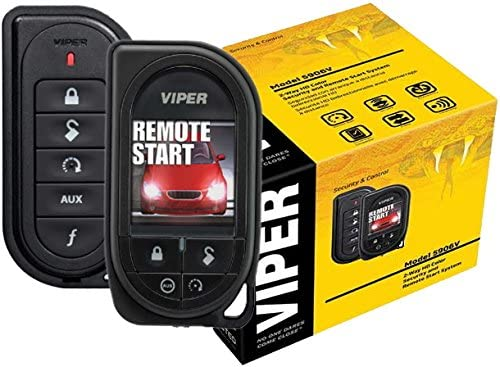
\includegraphics[width=\textwidth]{../latex/images/viper_5906V_1.jpg}
					\caption{Image of viper alarm}
				\end{figure}
			\end{columns}
		\end{block}
	\end{frame}

	\subsection{Carlock}
	\begin{frame}
		\frametitle{Carlock Car Alarm Features}
		\begin{block}{Carlock Car Alarm Features}
			\begin{columns}[c]
				\column{.35\textwidth}
				\begin{itemize}
					\item GPS Tracking.
					\item Lock/Unlock Car.
					\item Speed Status.
					\item Mobile Application.
					\item Car Battery Status Reporter.
					\item Configuring using OBD (On-board diagnostics).
				\end{itemize}
				\column{.55\textwidth}
				\begin{figure}[!h]
					\centering
					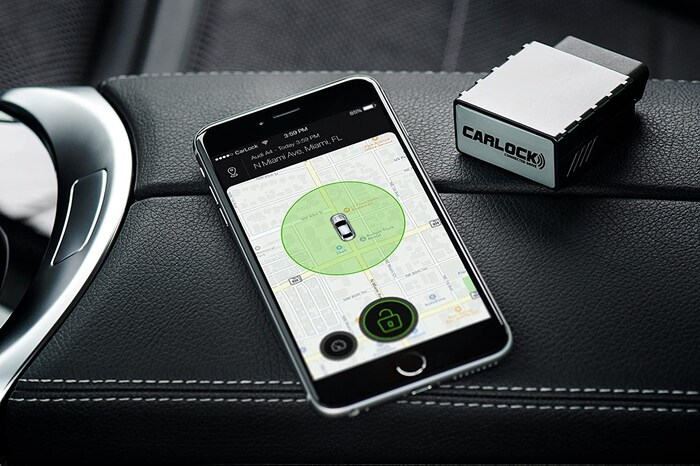
\includegraphics[width=\textwidth]{../latex/images/carlock-main-module.jpeg}
					\caption{Image of Carlock Alarm}
				\end{figure}
			\end{columns}
		\end{block}
	\end{frame}

	\section{Features}
	\begin{frame}
		\frametitle{Cardian Car Alarm Features}
		\begin{block}{Highlighted Features}
			\begin{itemize}
				\item GPS Tracking.
				\item Controling Remote over 1.5Km Range.
				\item Cross Platform Application.
				\item Car Status Reporter.
				\item Panic Mode.
				\item Etc.
			\end{itemize}
		\end{block}
	\end{frame}

	\section{Software Methodology}
	\begin{frame}
	\frametitle{Software Methodology}
	\begin{block}{Software Methodology}
		\begin{itemize}
			\item Kanban.
			\item Activity Diagram.
			\item Project Structure.
		\end{itemize}
	\end{block}
	\end{frame}

	\subsection{Kanban}
	\begin{frame}
	\frametitle{Software Methodology}
	\begin{block}{Kanban}
		\begin{columns}[c]
			\column{.35\textwidth}
			\begin{itemize}
				\item Agile.
				\item Personal Kanban.
				\item Github Projects.
				\item \url{https://github.com/users/0smr/projects/4}.
			\end{itemize}
			\column{.55\textwidth}
			\begin{figure}[!h]
				\centering
				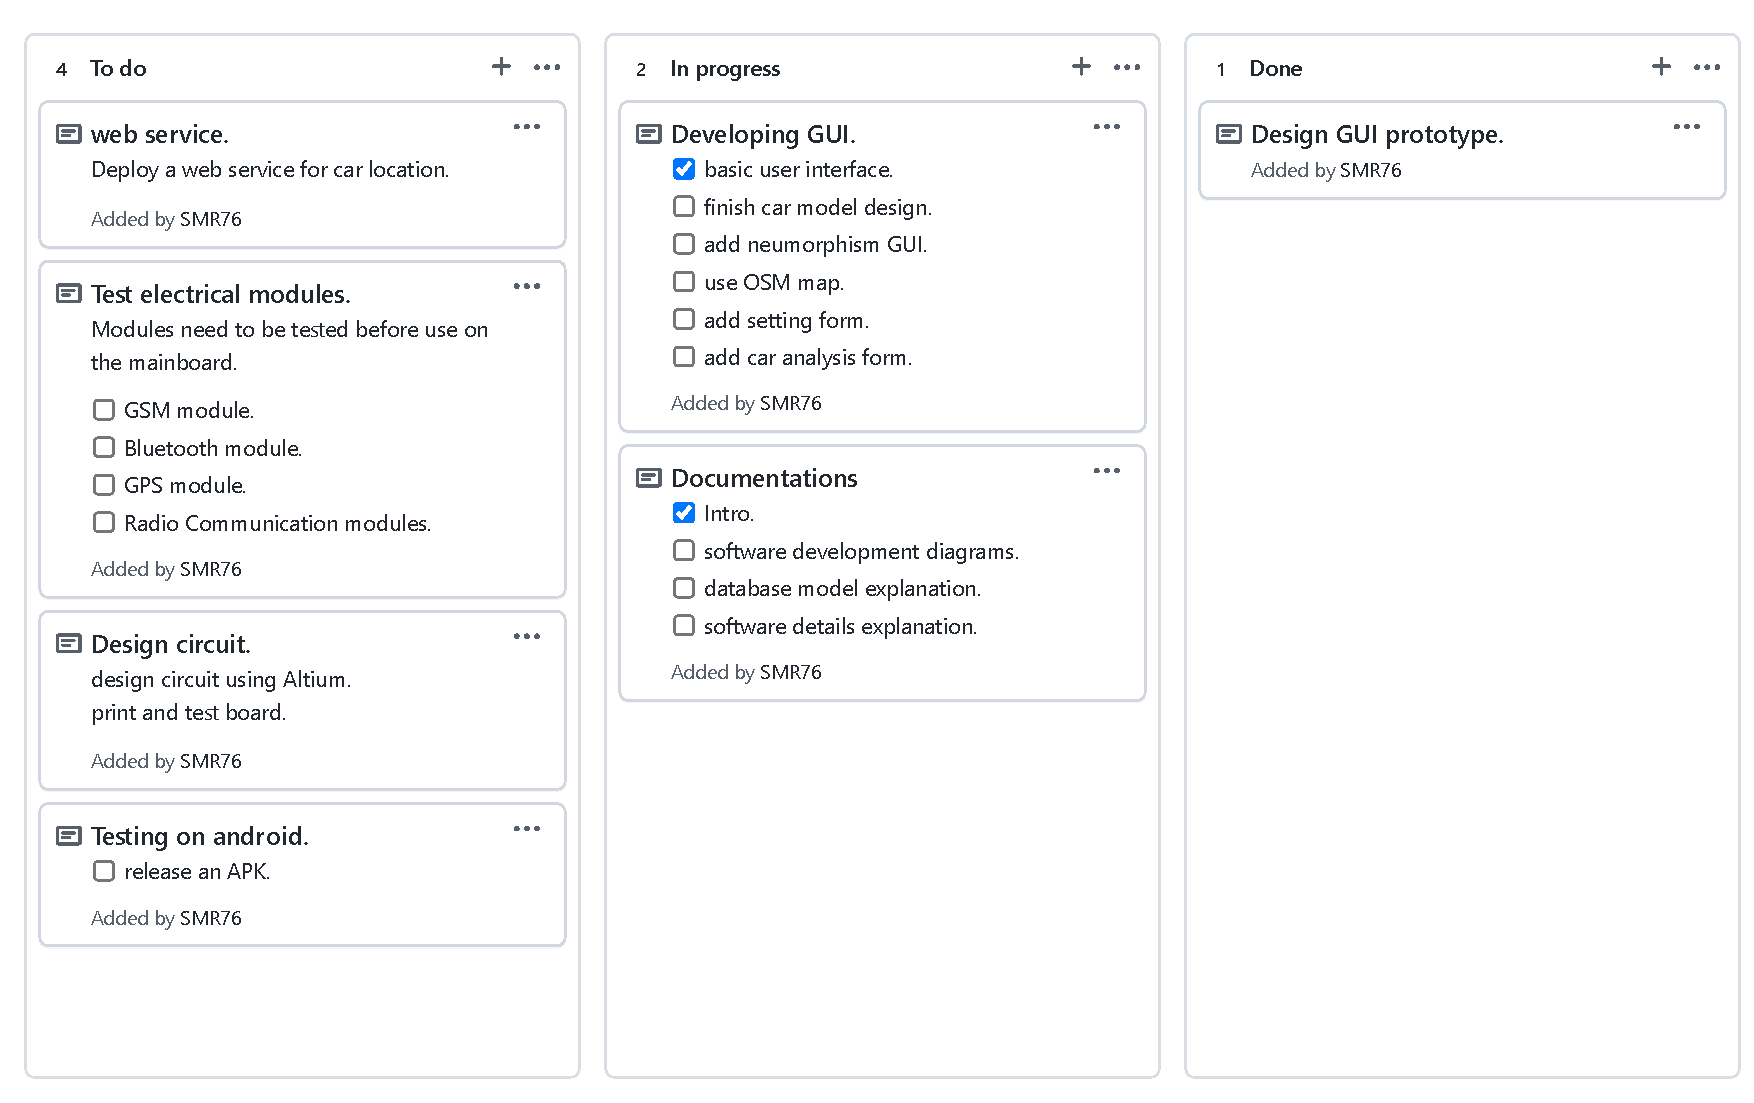
\includegraphics[width=\textwidth]{../latex/images/kanban-board.pdf}
				\caption{Image from Github Projects.}
			\end{figure}
		\end{columns}
	\end{block}
	\end{frame}

	\subsection{Activity}
	\begin{frame}
	\frametitle{Software Methodology}
	\begin{block}{Activity}
		\begin{columns}[c]
			\column{.35\textwidth}
			\begin{itemize}
				\item Activity Diagram.
			\end{itemize}
			\column{.55\textwidth}
			\begin{figure}[!h]
				\centering
				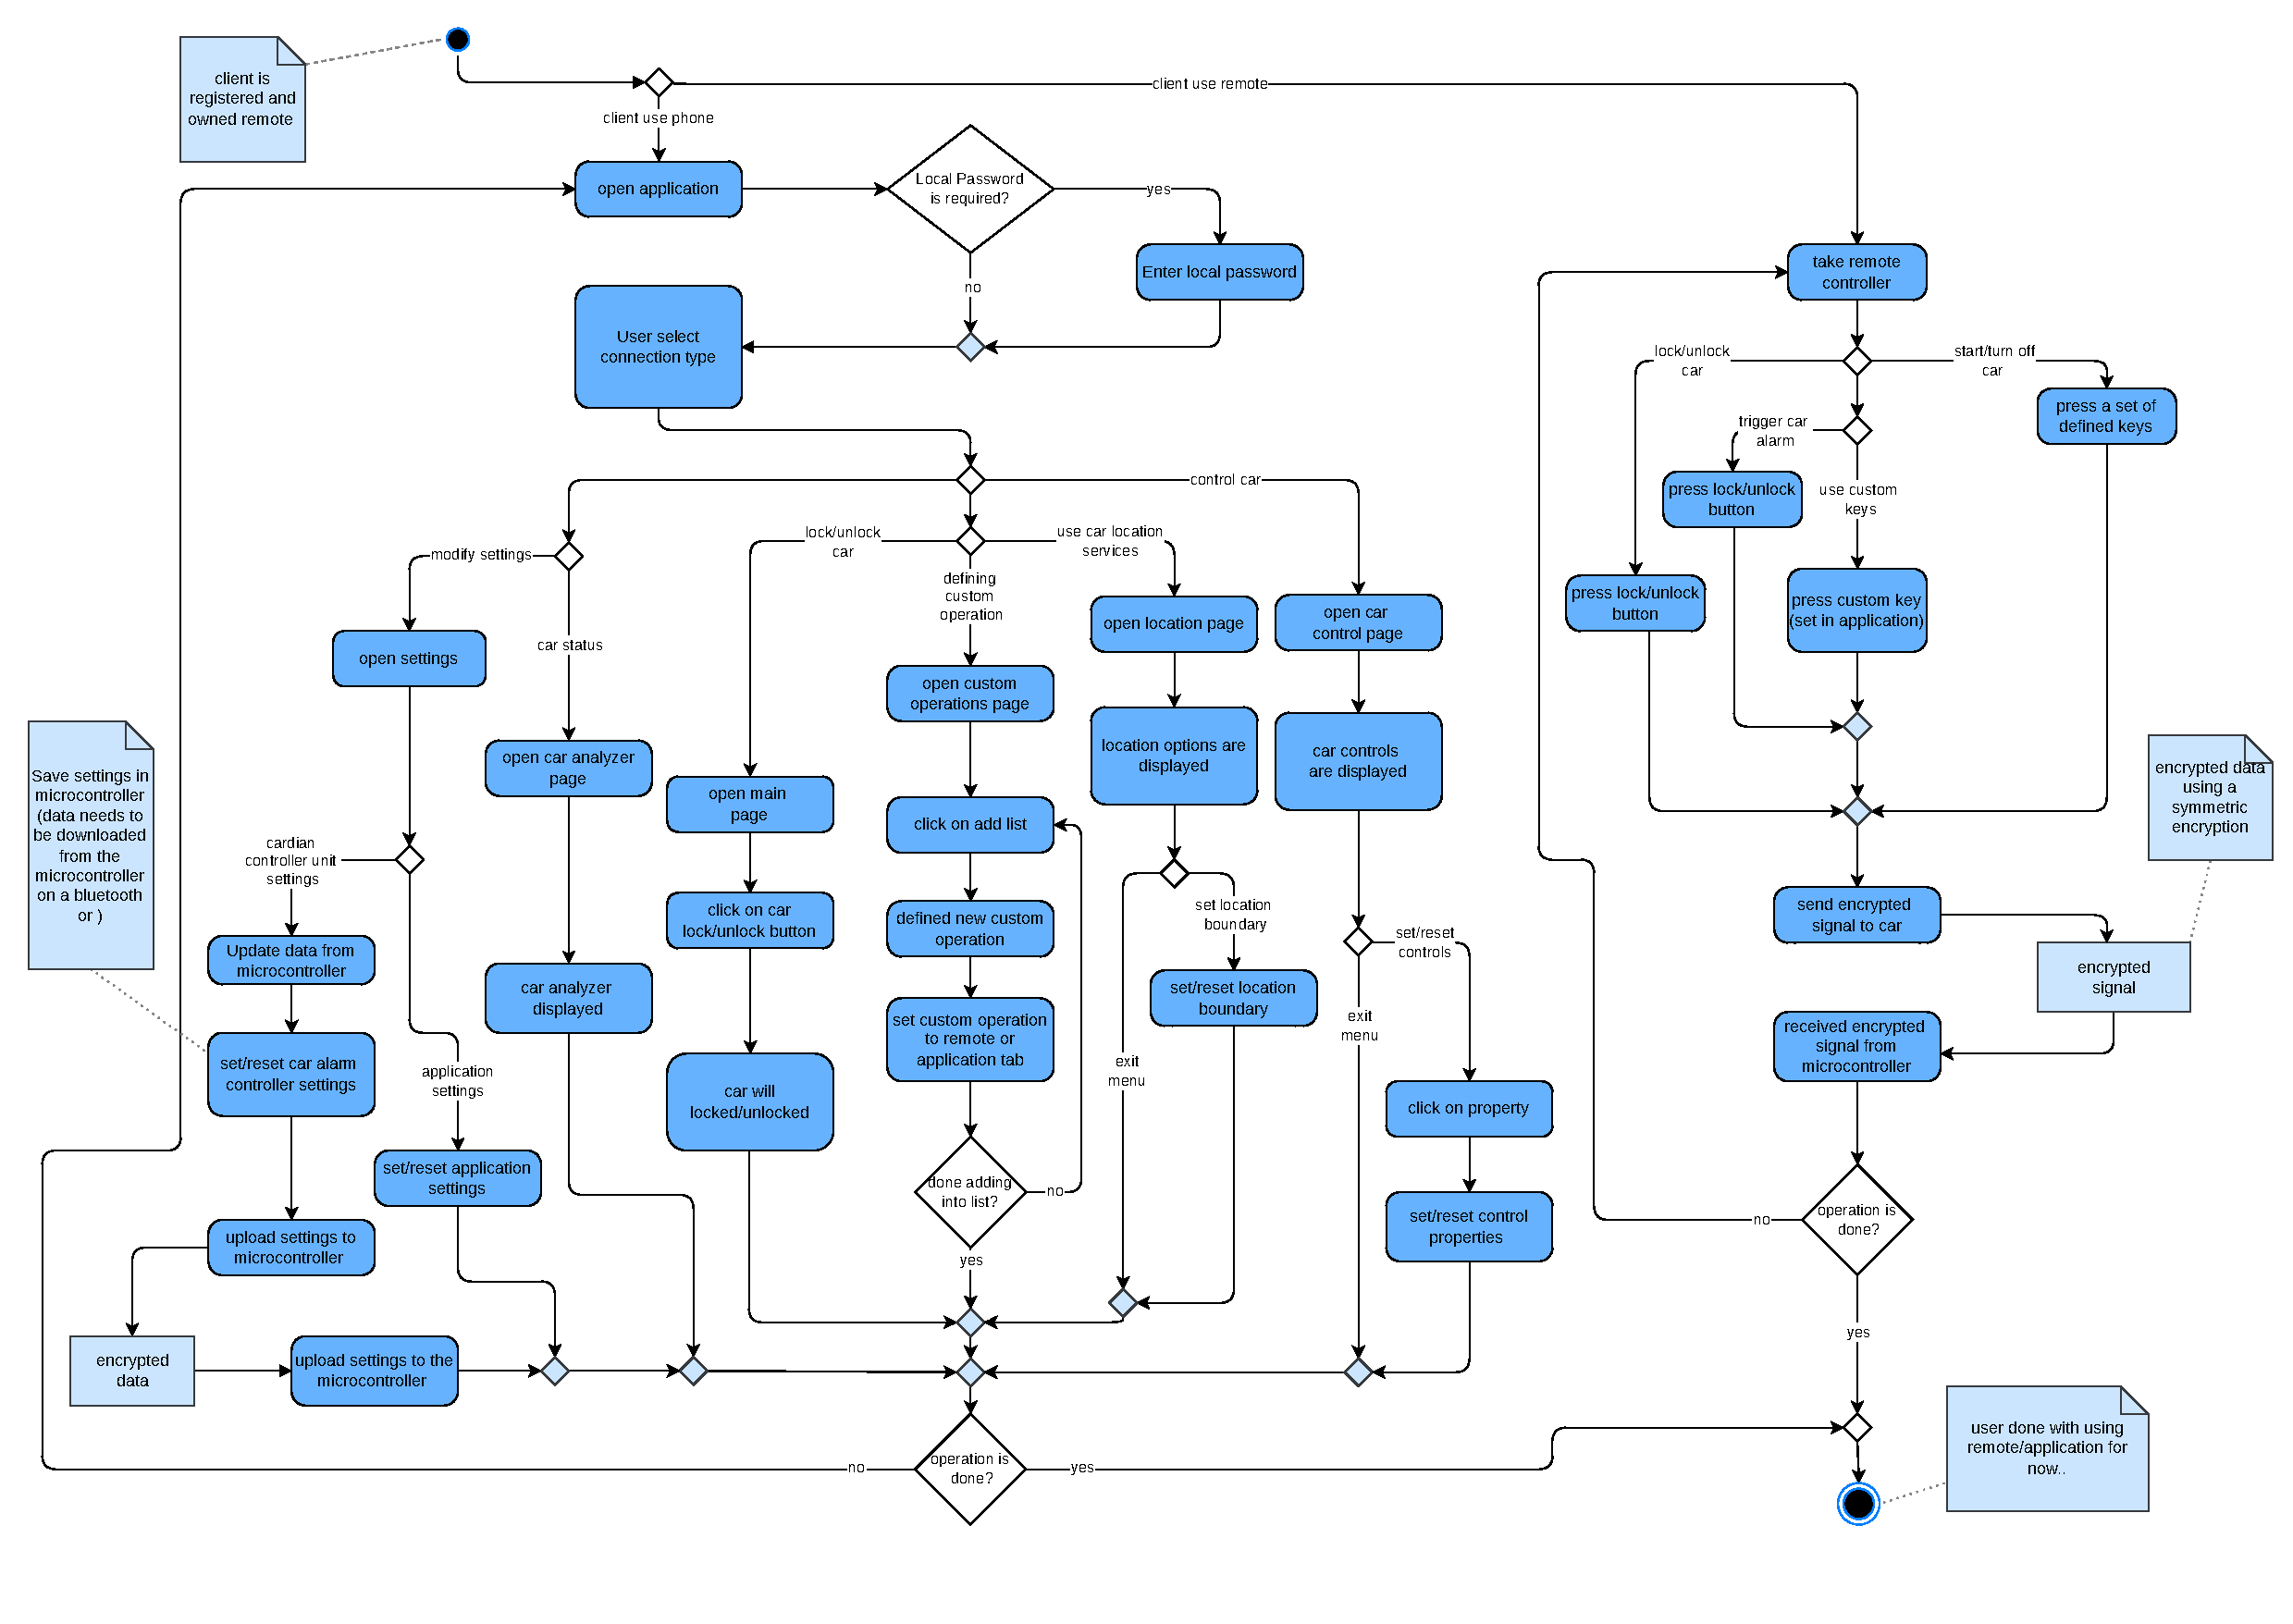
\includegraphics[width=\textwidth]{../diagrams/activity-diagram.pdf}
				\caption{Cardian Activity Diagram}
			\end{figure}
		\end{columns}
	\end{block}
	\end{frame}

	\subsection{Structure}
	\begin{frame}
	\frametitle{Software Methodology}
	\begin{block}{Project Structure}
		\begin{columns}[c]
			\column{.35\textwidth}
			\begin{itemize}
				\item Project Structure Diagram.
			\end{itemize}
			\column{.55\textwidth}
			\begin{figure}[!h]
				\centering
				\includegraphics[width=\textwidth]{../diagrams/project-structure.pdf}
				\caption{Cardian Project Structure}
			\end{figure}
		\end{columns}
	\end{block}
	\end{frame}

	\section{Database}
	\begin{frame}
	\frametitle{Database Structure}
	\begin{block}{Database Structure}
		\begin{itemize}
			\item MySQL.
			\item Diagram.
			\item Events.
		\end{itemize}
	\end{block}
	\end{frame}

	\subsection{Diagram}
	\begin{frame}
		\frametitle{Database}
		\begin{block}{Database Diagram}
			\begin{columns}[c]
				\column{.45\textwidth}
				\begin{itemize}
					\item Database Diagram.
				\end{itemize}
				\column{.45\textwidth}
				\begin{figure}[!h]
					\centering
					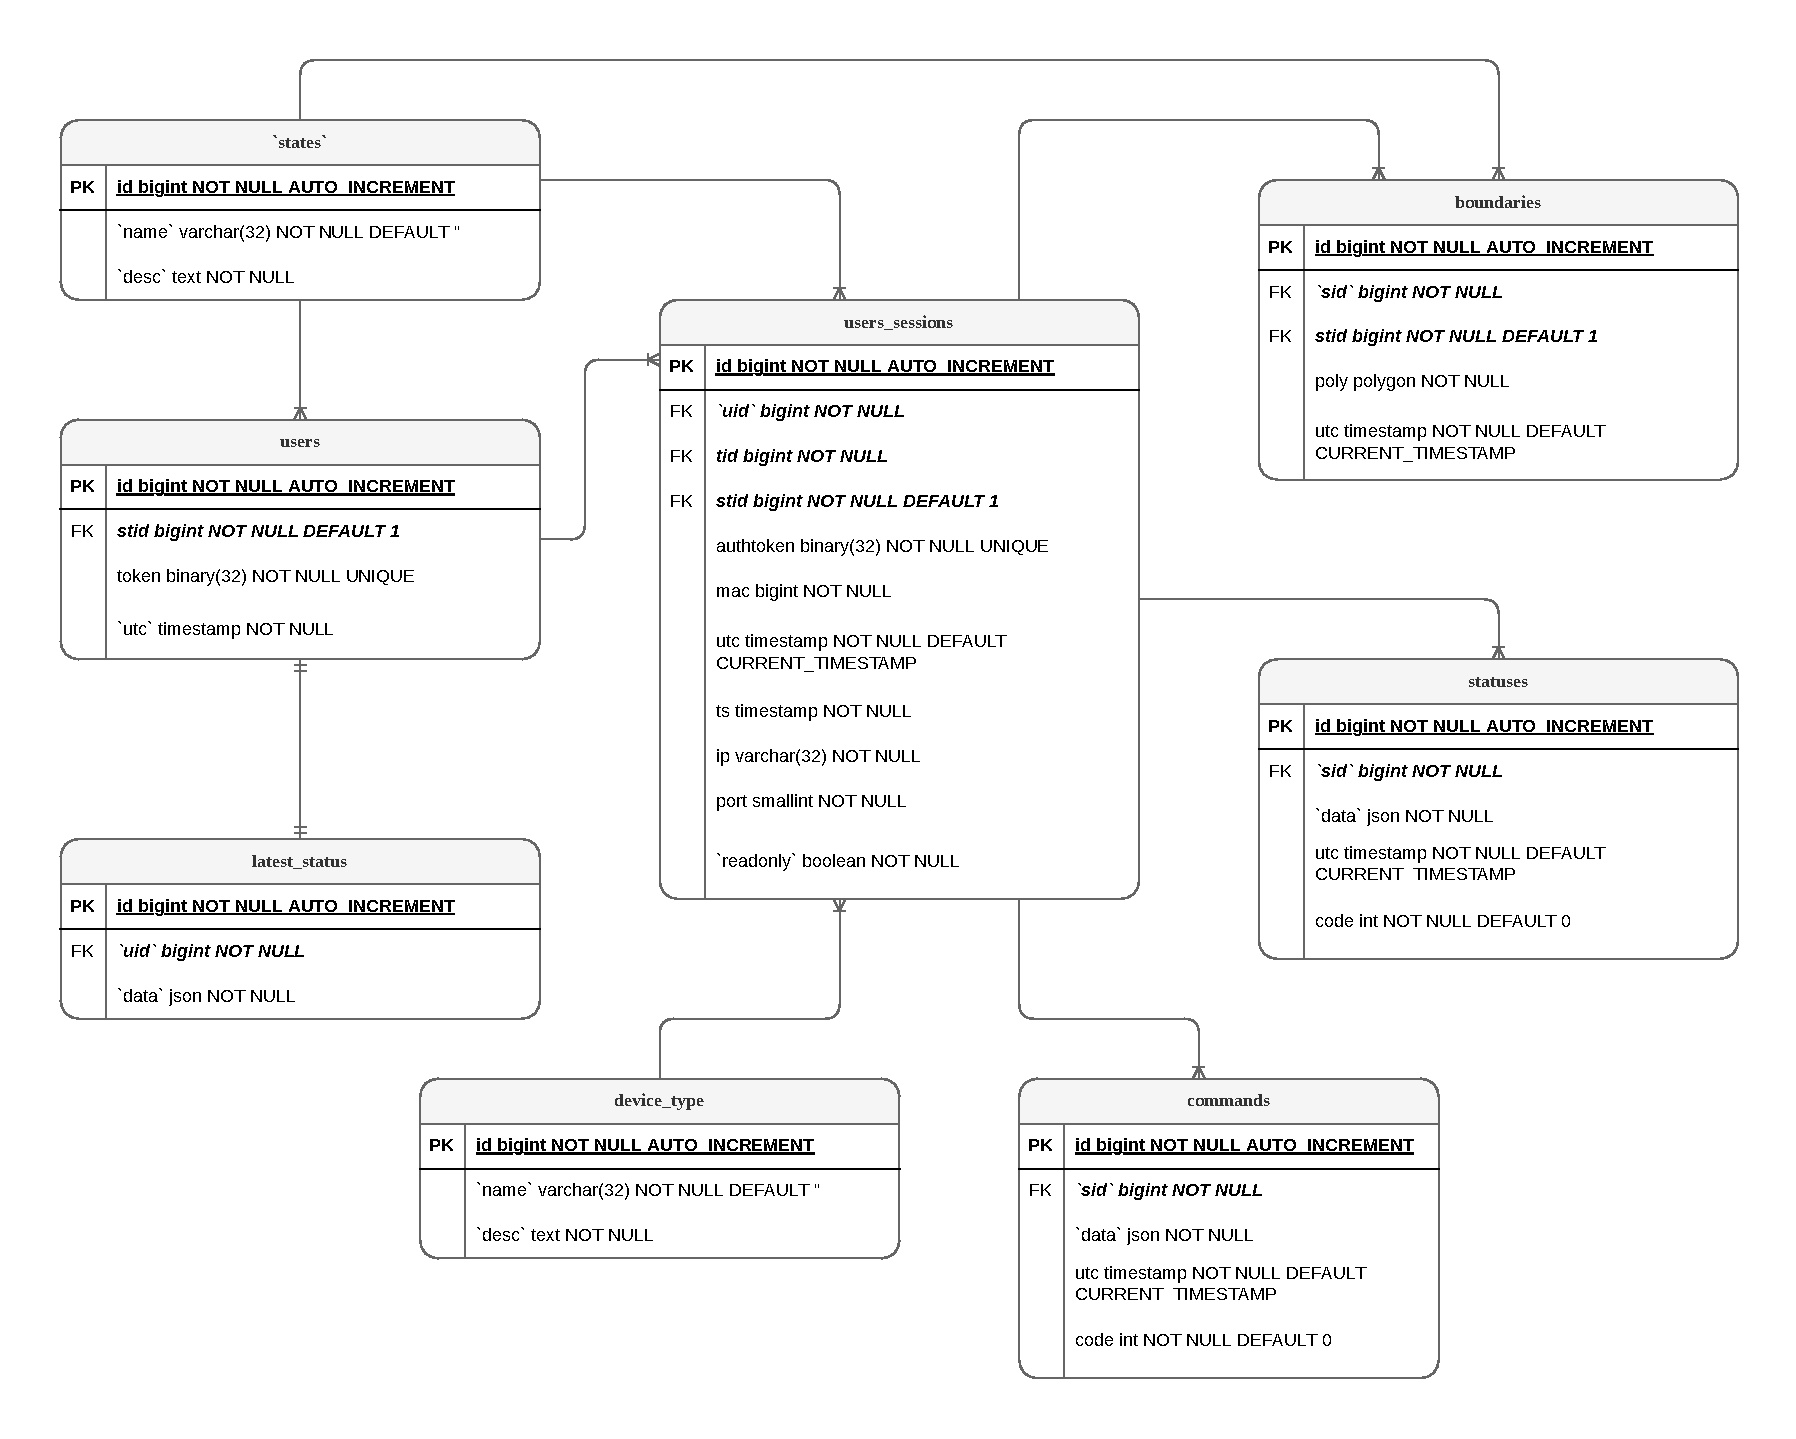
\includegraphics[width=\textwidth]{../diagrams/database.pdf}
					\caption{Database diagram image}
				\end{figure}
			\end{columns}
		\end{block}
	\end{frame}

	\section{Software Application}
	\begin{frame}
		\frametitle{Application}
		\begin{block}{Application}
			\begin{itemize}
				\item Qt Cross Platform Application.\cite{QtQML51548:online}
				\item Telegram as an inspiration.
				\item Server Side GraphQL using PHP.\cite{GraphQL:online}
			\end{itemize}
		\end{block}
	\end{frame}

	\subsection{Qt Cross Platform Application}
	\begin{frame}
		\frametitle{Application}
		\begin{block}{Qt Cross Platform Application}
			\begin{columns}[c]
				\column{.35\textwidth}
				\begin{itemize}
					\item QML.
					\item Veqtor.
					\item OpenGL shaders.
				\end{itemize}
				\column{.55\textwidth}
				\begin{figure}[!h]
					\centering
					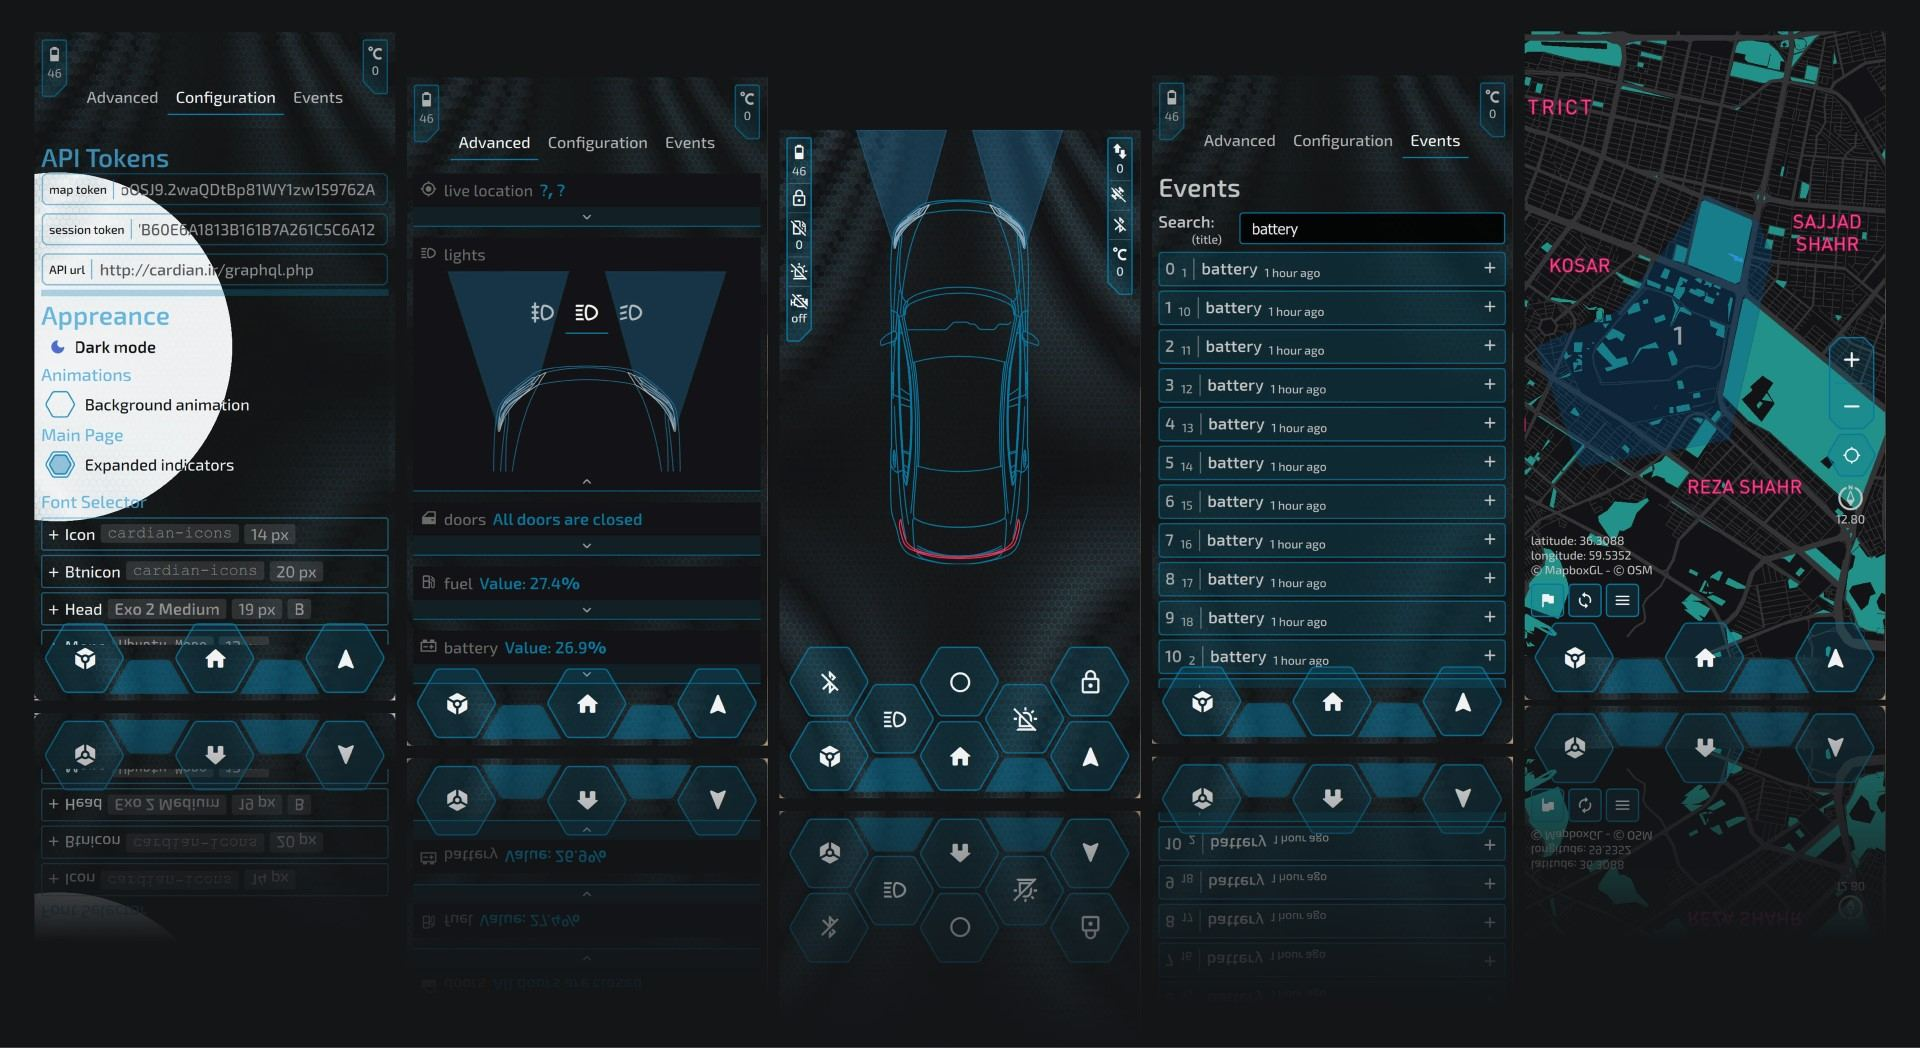
\includegraphics[width=\textwidth]{../latex/images/preview-dark.jpeg}
					\caption{Image of application}
				\end{figure}
			\end{columns}
		\end{block}
	\end{frame}

	\subsection{GraphQL Web Service}
	\begin{frame}
		\frametitle{GraphQL}
		\begin{block}{GraphQL}
			\begin{itemize}
				\item Php.
				\item GraphQL.
				\item webonyx/graphql.
			\end{itemize}
		\end{block}
	\end{frame}

	\section{Hardware}
	\begin{frame}
		\frametitle{Hardware}
		\begin{block}{Hardware}
			\begin{itemize}
				\item Remote.
				\item Main-Board.
			\end{itemize}
		\end{block}
	\end{frame}

	\subsection{Remote}
	\begin{frame}
		\frametitle{Hardware}
		\begin{block}{Remote}
			\begin{itemize}
				\item Arduino.
				\item HM-TRP.
				\item OLED Display.
			\end{itemize}
		\end{block}
	\end{frame}

	\subsection{Main Board}
	\begin{frame}
		\frametitle{Hardware}
		\begin{block}{Main Board}
			\begin{columns}[c]
				\column{.35\textwidth}
				\begin{itemize}
					\item STM32F103C8T6.
					\item SIM800L.
					\item NEO6MV2.
					\item HM-TRP.
				\end{itemize}
				\column{.55\textwidth}
				\begin{figure}[!h]
					\centering
					\includegraphics[width=\textwidth]{../latex/images/main-hardware-schematic.pdf}
					\caption{Main Hardware Schematic}
				\end{figure}
			\end{columns}
		\end{block}
	\end{frame}

	\section{Conclusion}
	\begin{frame}
		\frametitle{Conclusion}
		\begin{itemize}
			\item Market.
			\item GPT Like AI.
			\item Region Constraints.
		\end{itemize}
	\end{frame}

	\section*{References}
	\begin{frame}
		\frametitle{References}
		\nocite{*}
		\bibliographystyle{ieeetr}
		\bibliography{reference}
	\end{frame}

	\section*{Ending}
	\begin{frame}
		\huge{\centerline{Thanks for attention}}
	\end{frame}
\end{document}